\documentclass{article}
\usepackage{tikz}
\usepackage{amsmath,amsfonts,amssymb}
\usetikzlibrary{automata, shapes,arrows,positioning,calc}
\usepackage{hyperref}
\usepackage[margin=1in]{geometry}
\usepackage{graphicx}
\usepackage{float}
\usepackage{amsmath}
\usepackage{amssymb}
\usepackage{amsthm}
\usepackage{xfrac}
%if youre copying this make sure you have all the packages installed and get rid of the image near the bottom (it has a local path)
%links work as of december 17th, 2024
\begin{document}
\newgeometry{margin=0.1in} 

\begin{center}
  \large
  \textbf{Flowchart inspired (first page mostly copied from) by:} GOAT EngSci \href{https://xueqilin.me/engsci-2t4/esc194/lectures/flowchart.pdf}{QILIN XUE!!!} \\
  \textbf{Derivations and examples mostly taken from:} lecture or \href{https://tutorial.math.lamar.edu/}{Paul's Online Math Notes} \\
\end{center}

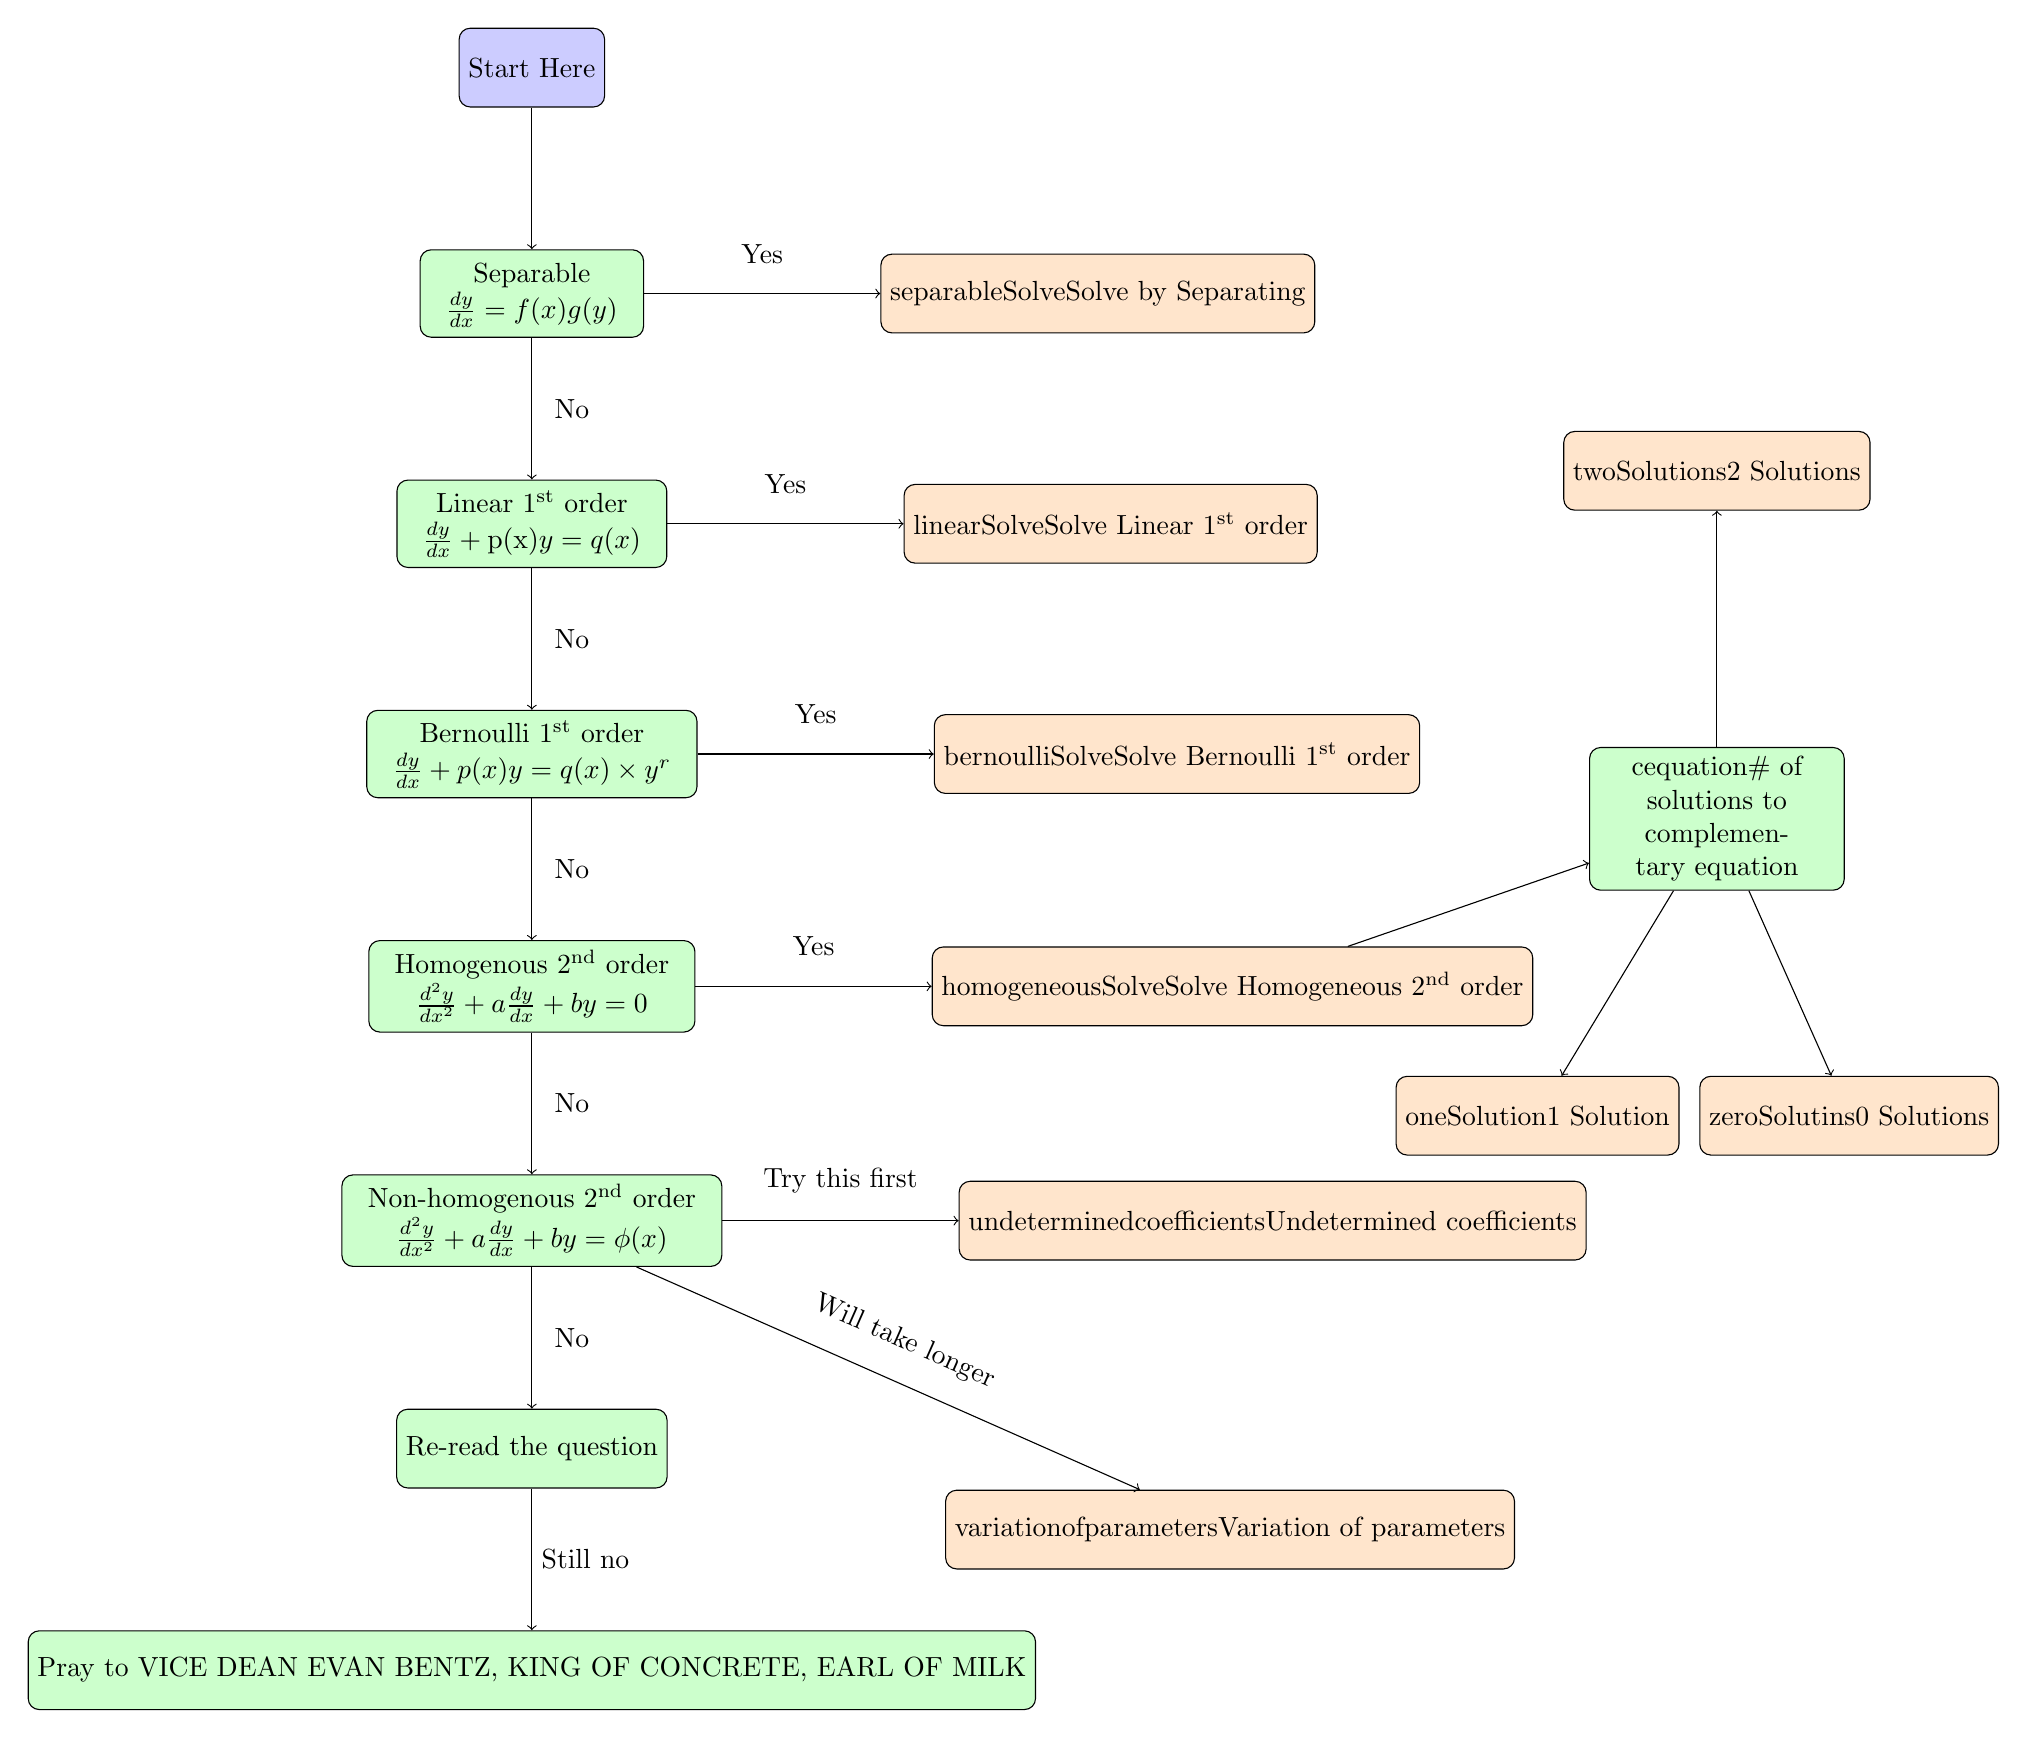
\begin{tikzpicture}[node distance=1.8cm, auto, every node/.style={rectangle, minimum size=1cm}]
  \node (start) [rectangle, rounded corners, draw, fill=blue!20] {Start Here};
  
  \node (separable) [rectangle, rounded corners, draw, fill=green!20, below=of start] {\begin{tabular}{c}Separable\\$\frac{dy}{dx} = f(x)g(y)$\end{tabular}};
  \node (linear) [rectangle, rounded corners, draw, fill=green!20, below=of separable] {\begin{tabular}{c}Linear $1^{\rm st}$ order\\$\frac{dy}{dx} + \text{p(x)}y=q(x)$\end{tabular}};
  \node (bernoulli) [rectangle, rounded corners, draw, fill=green!20, below=of linear] {\begin{tabular}{c}Bernoulli $1^{\rm st}$ order\\$\frac{dy}{dx} + p(x)y=q(x)\times y^r$\end{tabular}};
  \node (homogeneous) [rectangle, rounded corners, draw, fill=green!20, below=of bernoulli] {\begin{tabular}{c}Homogenous $2^{\rm nd}$ order\\$\frac{d^2y}{dx^2} + a\frac{dy}{dx} + by = 0$\end{tabular}};
  \node (nonhomogeneous) [rectangle, rounded corners, draw, fill=green!20, below=of homogeneous] {\begin{tabular}{c}Non-homogenous $2^{\rm nd}$ order\\$\frac{d^2y}{dx^2} + a\frac{dy}{dx} + by = \phi(x)$\end{tabular}};
    \node (end) [rectangle, rounded corners, draw, fill=green!20, below=of nonhomogeneous] {Re-read the question};
    \node (end2) [rectangle, rounded corners, draw, fill=green!20, below=of end] {Pray to VICE DEAN EVAN BENTZ, KING OF CONCRETE, EARL OF MILK};

  \node (separableSolve) [rectangle, rounded corners, draw, fill=orange!20, right=3cm of separable] 
    {\hyperlink{separableSolve}{Solve by Separating}};
  \node (linearSolve) [rectangle, rounded corners, draw, fill=orange!20, right=3cm of linear] 
    {\hyperlink{linearSolve}{Solve Linear $1^{\rm st}$ order}};
  \node (bernoulliSolve) [rectangle, rounded corners, draw, fill=orange!20, right=3cm of bernoulli] 
    {\hyperlink{bernoulliSolve}{Solve Bernoulli $1^{\rm st}$ order}};  
  \node (homogeneousSolve) [rectangle, rounded corners, draw, fill=orange!20, right=3cm of homogeneous] 
    {\hyperlink{homogeneousSolve}{Solve Homogeneous $2^{\rm nd}$ order}};
  \node (variationofparameters) [rectangle, rounded corners, draw, fill=orange!20, below right=4cm of nonhomogeneous, align=center] 
    {\hyperlink{variationofparameters}{Variation of parameters}}; 
  \node (undeterminedcoefficients) [rectangle, rounded corners, draw, fill=orange!20, right=3cm of nonhomogeneous] 
    {\hyperlink{undeterminedcoefficients}{Undetermined coefficients }};  

  \node (complementary) [rectangle, rounded corners, draw, fill=green!20, above right=1cm of homogeneousSolve, text width=3cm, align=center] {\hyperlink{cequation}{\# of solutions to complementary equation}};
  \node (twoSolutions) [rectangle, rounded corners, draw, fill=orange!20, above=3cm of complementary] {\hyperlink{twoSolutions}{2 Solutions}};
  \node (oneSolution) [rectangle, rounded corners, draw, fill=orange!20,below=3cm of complementary, below left= 2.35cm and -1.15cm of complementary] {\hyperlink{oneSolution}{1 Solution}};
  \node (zeroSolutions) [rectangle, rounded corners, draw, fill=orange!20, right=0.25 cm of oneSolution] {\hyperlink{zeroSolutins}{0 Solutions}};


  % Arrows
  \draw [->] (start) -- (separable);
  \draw [->] (separable) -- node {No} (linear);
  \draw [->] (linear) -- node {No} (bernoulli);
  \draw [->] (bernoulli) -- node {No} (homogeneous);
  \draw [->] (homogeneous) -- node {No} (nonhomogeneous);
  \draw [->] (homogeneousSolve) -- (complementary);
  \draw [->] (complementary) -- (twoSolutions);
  \draw [->] (complementary) -- (oneSolution);
  \draw [->] (complementary) -- (zeroSolutions);
  \draw [->] (nonhomogeneous) -- node {No} (end);
  \draw [->] (end) -- node {Still no} (end2);

  \draw [->] (separable) -- node {Yes} (separableSolve); 
  \draw [->] (linear) -- node {Yes} (linearSolve);
  \draw [->] (bernoulli) -- node {Yes} (bernoulliSolve);
  \draw [->] (homogeneous) -- node {Yes} (homogeneousSolve);
  \draw [->] (nonhomogeneous) -- node {Try this first} (undeterminedcoefficients);
  \draw [->] (nonhomogeneous) -- node[midway, sloped, above] {Will take longer} (variationofparameters);
\end{tikzpicture}
\restoregeometry 
\newpage 

\hypertarget{separableSolve}{
  \section*{Separable Differential Equations}
  \subsection*{Background info} 
  If you have an equation like $\frac{dy}{dx} = xy$, pretend $\frac{dy}{dx}$ is a fraction. Rearrange so that you get all the $y$ terms on one side and all the $x$ terms on the other. Then integrate with respect to the variable on each side. The answer will probably be explicit, but could be implicit; if so just leave it like that.
  \subsection*{Example:}
  \noindent \textbf{Problem:} \\[6pt]
  $y' = \frac{xy^3}{\sqrt{1+x^2}}, \quad y(0) = -1$ \\[6pt]
  \textbf{Steps:}\\[6pt]
  $y'$ is $\frac{dy}{dx}$, then separate the variables:
	\begin{align*}
	\frac{dy}{dx} &= \frac{xy^3}{\sqrt{1+x^2}} \\
	\frac{dy}{y^3} &= \frac{x}{\sqrt{1+x^2}} \, dx 
	\end{align*}
	Integrate! (u-sub for the right side)
	\begin{align*}
	\int \frac{dy}{y^3} &= \int \frac{x}{\sqrt{1+x^2}} \, dx \\
	-\frac{1}{2y^2} &= \sqrt{1+x^2} + C 
	\end{align*}
	Apply initial condition to find $C$:
	\begin{align*}
	-\frac{1}{2(-1)^2} &= \sqrt{1+0^2} + C \\
	-\frac{1}{2} &= 1 + C \\
	C &= -\frac{3}{2}
	\end{align*}
	Find explicit solution for y(x)
	\begin{align*}
	-\frac{1}{2y^2} &= \sqrt{1+x^2} - \frac{3}{2} \\
	\frac{1}{y^2} &= 3 - 2\sqrt{1+x^2} \\
	y^2 &= \frac{1}{3 - 2\sqrt{1+x^2}} \\
	y &= \pm \sqrt{\frac{1}{3 - 2\sqrt{1+x^2}}}
	\end{align*}
	Note that given the initial condition, we only take the negative root. Also note that the domain of x is restricted.
  \subsection*{Sample Problem: (Stewart 9.3.18)}
  $\frac{dL}{dt} = kL^2 \ln t, \quad L(1) = -1$ 
}
\hypertarget{linearSolve}{
  \section*{Linear $1^{\rm st}$ Order Differential Equations}
  \subsection*{Background info:} 
  The equation has to be in this form $\frac{dy}{dx} + p(x)y=q(x)$. Assume there is some function $\mu(x)$ (the integrating factor) has the property $\mu(x) p(x)= \mu'(x)$ (it later turns out that $\mu(x) = e^{\int p(t)dt}$). \newline
  Multiply through by $\mu(x)$ to get $\mu(x)\frac{dy}{dx} + \mu'(x)y=\mu(x)q(x)$. The left hand side of this equation is just the product rule of $(\mu(x)y(x))'$, so the equation becomes $(\mu(x)y(x))' = \mu(x)q(x)$. Integrate both sides \textbf{and keep the constant of integration from this step onwards}. \newline
  Isolate for $y(t)$ to get the solution to the equation:
\begin{equation*}
y(t) = \frac{\int \mu(t)q(t) dt - c}{\mu(t)}
\end{equation*}
where $\mu(x) = e^{\int p(t)dt}$. Note the sign of the constant doesn't matter.
  \subsection*{Example:}
  \textbf{Problem:}\\[6pt]
  $\frac{dv}{dt} = 9.8 - 0.196v, \quad v(0) = 48$ \\[6pt]
  \textbf{Steps:}\\[6pt]
  $p(t) = 0.196$ and $q(t) = 9.8$
	$\mu(t) = e^{\int p(t) \, dt} = e^{\int 0.196 \, dt} = e^{0.196t}$\newline
	Multiply through to get $\frac{d}{dt} (e^{0.196t} v) = 9.8e^{0.196t}$\newline
	Integrate both sides and divide out to find explicit solution for v: $v(t) = 50 + Ce^{-0.196t}$ \newline
	Use initial condition to find that $C = -2$, so final answer becomes: $v(t) = 50 - 2e^{-0.196t}$
}
\hypertarget{bernoulliSolve}{
  \section*{Bernoulli $1^{ \rm st}$ Order Differential Equations}
  \subsection*{Background info} 
  Given a differential equation in this form $\frac{dy}{dx} + p(x)y=q(x)y^n$, where $n \ne 0 \text{ or } 1$ (because thats just a linear 1st order differential equation (see above). Divide through by $y^n$ and make the substitution $v=y^{1-n}$. Note $\frac{dv}{dx} = (1-n)y^{-n}\frac{dy}{dx}$, so the equation can be rearranged to 
\begin{equation*}
\frac{v'(x)}{1-n} + p(x)v=q(x)
\end{equation*}
which is just a linear differential equation (with a different variable!!).
  \subsection*{Example:}
  \textbf{Problem:}\\[6pt]
  $y' + \frac{4}{x} y = x^3 y^2, \quad y(2) = -1$\\[6pt]
  \textbf{Steps:}\\[6pt]
   Let $v = y^{1 - 2} = y^{-1}$ and thus $y' = -v^{-2} v'$\newline
   Substitute to get $-v^{-2} v' + \frac{4}{x} v^{-1} = x^3 v^{-2}.$\newline
   Divide through to get a linear first order equation which has an integrating factor of $e^{\int -\frac{4}{x} \, dx} = e^{-4 \ln x} = x^{-4}$
	Multiply through to get $x^{-4}v =\int{-x^{-1}dx}$\newline
	Integrate both sides and divide out to find explicit solution for v: $v(x) = x^4(c-lnx)$ \newline
	We need an explicit solution for y and the value of c, so we'll find both. The equation for y becomes $y^{-1} = x^4(c-lnx)$. Applying the initial condition, we get $c= \ln 2 - \frac{1}{16}$
}
\hypertarget{homogeneousSolve}{
  \section*{Homogeneous $2^{\text{\rm nd}}$ Order Differential Equations}
  \subsection*{Background info:} 
  The equation should be in the form $ay'' + by' + cy = 0$.\newline 
  The \textbf{Principle of Superposition} states that if $y_1(x)$ and $y_2(x)$ are two linearly independent ``nice enough'' solutions (the Wronskian doesn't disappear or something like that. Irrelevant for 194), then the general solution to the differential equation is $y(x) = c_1y_1(x) + c_2y_2(x)$, where $c_1, c_2$ are some constants.\newline
}
\hypertarget{cequation}{
    \section*{Complementary equation}
    \subsection*{Background info:}
   	Set the polynomial to zero and make it a homogeneous equation. \textbf{Do NOT find the coefficients} 
}
\hypertarget{oneSolution}{
    \section*{Homogeneous $2^{nd}$ Order Differential Equations: One Solution}
    \subsection*{Background:}
    If there's only one real root, then if we try the method with two roots we get $y_1 = y_2$, which doesn't really work. Magic happens and then the solution becomes: 
  \begin{equation*}
  y(x) = c_1 e^{\sfrac{-bx}{2a}} + c_2 xe^{\sfrac{-bx}{2a}}
  \end{equation*}
    \subsection*{Sample Problem:}
    Solve the differential equation $y'' - 4y' + 4y = 0$.
}
\hypertarget{zeroSolutions}{
    \section*{Homogeneous $2^{\rm nd}$ Order Differential Equations: Zero Solutions}
    \subsection*{Background info:}
    If the roots are not real, use \textbf{Euler's formula:} $e^{i\theta} = \cos\theta + i\sin\theta$ (note you can (will) use the form where $\theta$ is negative, in that case, remember the even/odd behavior of sin/cos). The following equations use $\lambda = \frac{-b}{2a}$ and $\mu = \sqrt{b^2 - 4ac}$, where $\mu$ is just the real part (multiply by $i$). 
  \begin{align*}
	y_1(x) &= e^{(\lambda + \mu i)x} \quad \text{and} \quad y_2(x) = e^{(\lambda - \mu i)x} \\
	\\
	y_1(x) &= e^{\lambda x} e^{\mu i x} = e^{\lambda x} (\cos(\mu x) + i \sin(\mu x)) \\
	y_2(x) &= e^{\lambda x} e^{-\mu i x} = e^{\lambda x} (\cos(\mu x) - i \sin(\mu x))
  \end{align*}
  Add/subtract the two solutions together to get both solutions, and then you get:
  \begin{equation*}
  y(x) = c_1 e^{\lambda x} \cos(\mu x) + c_2 e^{\lambda x} \sin(\mu x)
  \end{equation*}
}
\hypertarget{twoSolutions}{
    \section*{Homogeneous $2^{nd}$ Order Differential Equations: Two Solutions}
    \subsection*{Backgroud info:}
 	  A likely candidate for $y(x)$ is something along the lines of $e^{rx}$, where $r$ is some constant. If that was the case, then by taking the derivative twice, the equation becomes $e^{rx}(ar^2 + br + c) = 0$. Since $e^{\text{something}}$ is never 0, the polynomial has to be zero at some point. Factor it to get the possible values of $r$, and then if they're real, plug in and you're done.
}
\hypertarget{undeterminedcoefficients}{
    \section*{Method of undetermined coefficients}
    \subsection*{Background info:}
		\begin{equation*}
		ay'' + by' + cy = g(x)
		\end{equation*}
		Similarlyish to solving for homogenous equations, the solution is going to be something along the lines of the solution to the complementary equation + the actual solution.
		\textbf{1. Guess $y_p$ based on $g(x)$:}
		\begin{itemize}
		  \item \textbf{Case 1:} $g(x)$ is a polynomial. 
		    Guess: $y_p = Ax^n + Bx^{n-1} + \dots + Cx + D$.
		    Even if there are not all the polynomial terms in the original g(x), there still has to be all of them in the equation.
		  \item \textbf{Case 2:} $g(x)$ is exponential ($e^{kx}$). 
		    Guess: $y_p = Ae^{kx}$.
		  \item \textbf{Case 3:} $g(x)$ is sine or cosine ($\sin(kx)$ or $\cos(kx)$). 
		    Guess: $y_p = A\cos(kx) + B\sin(kx)$, or something easier if it clearly cancels.
		\end{itemize}
		\textbf{Notes:}
		\begin{itemize}
		  \item If $g(x)$ combines functions, combine guesses.
		  \item If any $y_p$ term solves the homogeneous equation, multiply $y_p$ by $x$ (or $x^2$) until no term is a homogeneous solution.
		\end{itemize}
		Substitute $y_p$ and its derivatives into the differential equation, then equate coefficients to find the undetermined coefficients.
}
\hypertarget{variationofparameters}{
    \section*{Variation of parameters}
    \subsection*{Background info:}
    Same idea as undetermined coefficients. Start by assuming a particular solution of the form
	\begin{equation*}
	y_p(x) = u_1(x)y_1(x) + u_2(x)y_2(x) 
	\end{equation*}
	where $u_1(x)$ and $u_2(x)$ are functions to be determined. u is some made up thing so we can force it to follow $u_1' y_1 + u_2' y_2 = 0$
	Plugging and chugging, we get.
	\begin{align*}
		y_p' &= u_1' y_1 + u_2' y_2 + u_1 y_1' + u_2 y_2' \\
		y_p'' &= u_1' y_1' + u_2' y_2' + u_1 y_1'' + u_2 y_2'' \\
		\\
		a(u_1' y_1' &+ u_2' y_2' + u_1 y_1'' + u_2 y_2'')  + b(u_1 y_1' + u_2 y_2') + c(u_1 y_1 + u_2 y_2) = g(x) \\
		\\
		u_1(ay_1'' &+ by_1' + cy_1) + u_2(ay_2'' + by_2' + cy_2) + a(u_1' y_1' + u_2' y_2') = g(x)\\
		\end{align*} 
		Since $ay_1'' + by_1' + cy_1 = 0 \quad \text{and} \quad ay_2'' + by_2' + cy_2 = 0$ (solutions to complementary equation), we can simplify to 
		$a(u_1' y_1' + u_2' y_2') = g(x)$
Integrate and substitute as neccesary.
}
\section*{Relevant exam question}\label{123}
\subsection*{(a)}
Let $y_1(x)$ and $y_2(x)$ be two linearly independent solutions of 
\[y'' + ay' + by = 0\]
where $a$ and $b$ are constants. By proving that $W'(x) = -aW(x)$, show that either $W(x) = 0$ for all $x$ or $W(x) \neq 0$ for any $x$.
\begin{proof}
~\begin{enumerate}
\item \textbf{Derivative of the Wronskian:}
The Wronskian is defined as $W(x) = y_1(x)y_2'(x) - y_2(x)y_1'(x)$.  Differentiating with respect to $x$, we get:
\begin{align*}
W'(x) &= y_1'(x)y_2'(x) + y_1(x)y_2''(x) - y_2'(x)y_1'(x) - y_2(x)y_1''(x) \\
&= y_1(x)y_2''(x) - y_2(x)y_1''(x)
\end{align*}
\item \textbf{Using the differential equation:}
Since $y_1$ and $y_2$ are solutions to the differential equation $y'' + ay' + by = 0$, we have:
\begin{align*}
y_1''(x) &= -ay_1'(x) - by_1(x) \\
y_2''(x) &= -ay_2'(x) - by_2(x)
\end{align*}
Substituting these into the expression for $W'(x)$:
\begin{align*}
W'(x) &= y_1(x)[-ay_2'(x) - by_2(x)] - y_2(x)[-ay_1'(x) - by_1(x)] \\
&= -ay_1(x)y_2'(x) - by_1(x)y_2(x) + ay_2(x)y_1'(x) + by_2(x)y_1(x) \\
&= -a[y_1(x)y_2'(x) - y_2(x)y_1'(x)] \\
&= -aW(x)
\end{align*}
\item \textbf{Solving the differential equation for $W(x)$:}
The differential equation $W'(x) = -aW(x)$ has the solution:
$W(x) = W(0)e^{-ax}$
\item \textbf{Conclusion:}
Since $e^{-ax} \neq 0$ for all $x$, $W(x) = 0$ if and only if $W(0) = 0$. Therefore, either $W(x) = 0$ for all $x$, or $W(x) \neq 0$ for any $x$.
\end{enumerate}
\end{proof}
\subsection*{(b)}
Let $P(x)$ and $Q(x)$ be given, continuous functions. Let $y_1(x)$ and $y_2(x)$ be two solutions of 
\[y'' + P(x)y' + Q(x)y = 0\]
such that their Wronskian $W(x)$ never vanishes. Show that between two consecutive zeros of $y_1(x)$, there is one and only one zero of $y_2(x)$.
\begin{proof}
~\begin{enumerate}
\item \textbf{Rolle's Theorem:}
If a function $f(x)$ is continuous on $[a, b]$, differentiable on $(a, b)$, and $f(a) = f(b) = 0$, then there exists at least one $c \in (a, b)$ such that $f'(c) = 0$.
\item \textbf{Applying Rolle's Theorem to $y_1(x)$:}
Let $a$ and $b$ be consecutive zeros of $y_1(x)$, so $y_1(a) = y_1(b) = 0$.  As a solution to a second-order linear differential equation with continuous coefficients, $y_1(x)$ is continuous and differentiable. By Rolle's Theorem, there exists $c \in (a, b)$ such that $y_1'(c) = 0$.
\item \textbf{Using the Wronskian:}
At $x = c$, the Wronskian is:
\begin{align*}
W(c) &= y_1(c)y_2'(c) - y_2(c)y_1'(c) \\
&= y_1(c)y_2'(c) \quad (\text{since } y_1'(c) = 0)
\end{align*}
Since $W(c) \neq 0$ and $y_1(c) = 0$, we must have $y_2'(c) \neq 0$.
\item \textbf{Applying Rolle's Theorem to $y_2(x)$:}
If $y_2(a) = y_2(b) = 0$, then by Rolle's Theorem, there would exist $d \in (a, b)$ such that $y_2'(d) = 0$. But $y_2'(c) \neq 0$ and $c \in (a, b)$, so $y_2(x)$ cannot have two zeros between $a$ and $b$.
\item \textbf{Conclusion:}
We have shown that $y_2(x)$ cannot have two zeros between consecutive zeros of $y_1(x)$. Since the Wronskian never vanishes, $y_1(x)$ and $y_2(x)$ cannot have a common zero.  Therefore, there is one and only one zero of $y_2(x)$ between two consecutive zeros of $y_1(x)$.
\end{enumerate}
\end{proof}
\end{document}